\begin{figure}[t]
    \centering
    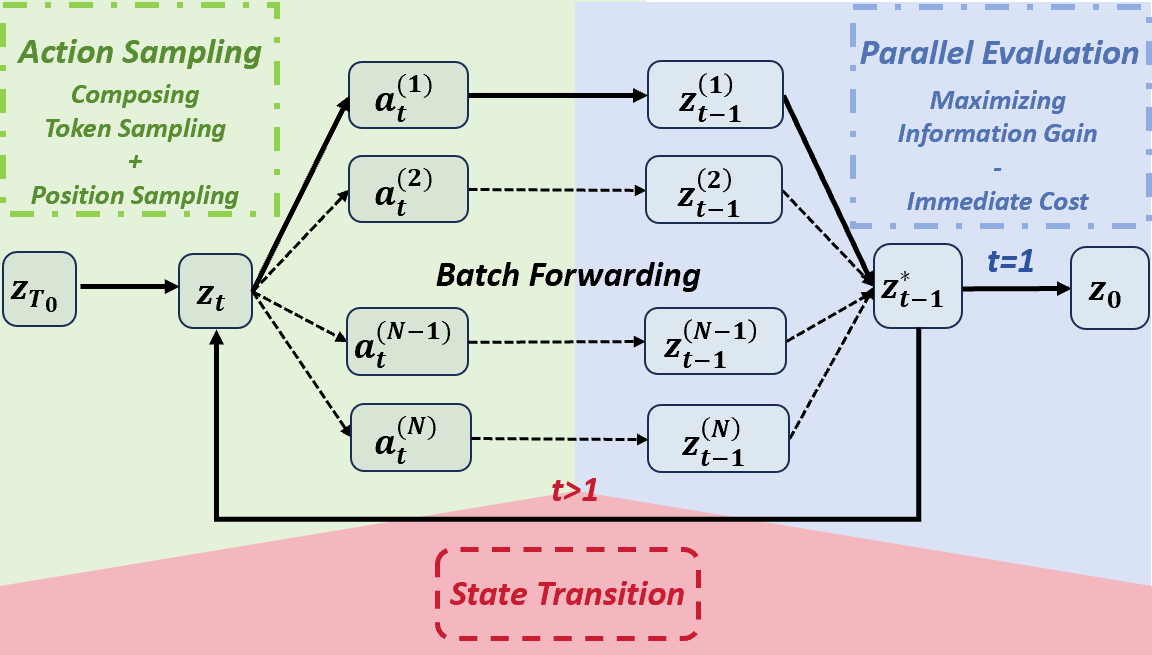
\includegraphics[width=1\linewidth]{workflow_v2.png}
    \caption{The Info-Gain Sampler workflow. Starting from state $z_{T_0}$, the sampler iteratively: (1) samples candidate actions, (2) evaluates $J_{\text{IG}} = \text{Immediate Cost} - \text{Information Gain}$ in parallel to select the optimal successor state $z_{t-1}^*$, and (3) executes the state transition until reaching the final sequence $z_0$.}
    \label{igp_workflow}
\end{figure}
